\documentclass[HardwareDesign/HardwareDesign_main.tex]{subfiles}
\begin{document}
\section{CupLight Hardware Design}
 I dette afsnit laves der overvejelser omkring det lys, der skal være under kopperne på Beer Pong bordet. Både lyset i al sin enkelthed men også hvordan lyset skal styres.
 
 
Før der dog kan laves et design, må der først og fremmest kigges på, hvilke krav der er til lyset. Af Kravsspecifikationen hives der følgende krav ud omkring lyset:
\begin{enumerate}
    \item Koplys skal kunne have forskellige farver.
    \item Hver enkelt koplys skal kunne styres individuelt, til at have sin egen farve.
\end{enumerate}
Da lyset skal styres af en controller pr. spillerside, så giver det umiddelbart også et krav om at alle led'er skal kunne styres med forholdsvis få pins på PSoC'en. 
\\Lyset skal kunne styres på en effektiv, men også billig måde, da det ville være spild af ressourcer at bruge al budgettet på bordet på at lave belysning frem for egentlig funktionalitet. Derfor besluttes der at bruge almindelige RGB-led'er, som kan købes på nettet forholdsvis billigt. Der findes også RGB-led'er der kan addresseres individuelt, men disse blev valgt fra, da de var for dyre. 
\\Der findes to typer RGB-led'er; Common Anode og Common Cathode. Da der ikke er klare fordele og ulemper mellem de to, vælges en RGB-led med Common Cathode, da den har nogle fordele i forhold til den styring, der laves dertil. 
\\Mere specifikt blev der til projektet valgt en RGB Led med vare nummeret: \textit{L-154A4SURKQBDZGW}\footnote{\href{http://www.farnell.com/datasheets/2046599.pdf?_ga=2.134869041.1755092500.1541003763-1168485423.1534934558}{RGB LED Datasheet}}. Denne LED består i princippet af 3 LED'er, en rød, en grøn og en blå. Derfor skal der til 3 af benene forbindes resistorer, men disse er nødvendigvis ikke samme størrelse, da LED'erne har forskellige elektroniske karakteristikker. For at finde størrelsen af resistorene bruges Ohms lov.
\begin{equation}
    R=\frac{U}{I}
\end{equation}
Til de elektroniske karakteristikker slås der op i databladet for LED'en. Her er man interesseret i strømmen gennem LED'erne, og hver enkelts Forward Voltage. Det findes at $I=20mA$, $V_R=1.95V$, $V_G=3.3V$ og $V_B=3.3V$. Det er nu muligt at finde de enkelte modstande for hver LED.

\begin{subequations}
        RGB Resistor Værdier:
\begin{align}
        R_{red}=\frac{V_{CC}-V_R}{I}=\frac{3.05V}{20mA}=152.5\Omega\\
        R_{green}=\frac{V_{CC}-V_G}{I}=\frac{1.7V}{20mA}=85\Omega\\
        R_{blue}=\frac{V_{CC}-V_B}{I}=\frac{1.7V}{20mA}=85\Omega
\end{align}
\end{subequations}

Da det er besluttet at hver Kop Holder, skal have 5 LED'er, så er det også relevant at kigge på, hvor meget effekt der bliver afsat i sådan en kopholder til LED'erne.
\begin{equation}
    P_{kop}=5\cdot V_{CC}\cdot I_{tot} = 5\cdot 5V\cdot 60mA = 1.5W
\end{equation}
Denne effekt er beregnet ud fra antallet af Led'er gange med spændingen, gange med den totale strøm gennem LED'en.

Til at slukke og tænde led'erne skal bruges en transistor og den transistor der er valgt er BC557B, der er en general purpose PNP transistor. Denne transistor er valgt, da den kan levere continous current på 100 mA. Dette er lige tilstrækkeligt, da hver transistor skal kunne levere strøm til 5 LED'er, hvilket giver collector current $I_C=20mA\cdot5=100mA$.
Da LED'erne skal tændes og slukkes med transistoren, så der skal også laves en beregning af den modstand, der skal forbindes til basen af transistoren.
Denne beregnes på følgende måde.
\begin{equation}
    R_B = \frac{V_C-V_{be}}{I_b}
\end{equation}

I databladet\footnote{https://www.onsemi.com/pub/Collateral/BC556B-D.PDF} findes det at transistoren er saturated når der trækkes $i_c=100mA$ og $i_b=5mA$, hvilket given en emitter/base spænding på $V_{be}=1V$. Det giver at formodstandens værdi er:
\begin{equation}
    R_B = \frac{5V-1V}{5\cdot 10^{-3} mA}=800\Omega
\end{equation}

Da der anvendes en transistor, vil der et spændingsfald over transistoren i forhold til supply spændingen kaldet $max(V_{CE})=0.65V$. Denne skal tages hensyn til i forbindelse med LED'erne, da det ændrer størrelsen på formodstanden lidt. Omregningen kan ses som:

\begin{subequations}
        RGB Resistor Værdier med hensyn til transistor:
\begin{align}
        R_{red}=\frac{V_{CC}-V_{CE}-V_R}{I}=\frac{2.4V}{20mA}=120\Omega\\
        R_{green}=\frac{V_{CC}-V_{CE}-V_G}{I}=\frac{1.05V}{20mA}=52.5\Omega\\
        R_{blue}=\frac{V_{CC}-V_{CE}-V_B}{I}=\frac{1.05V}{20mA}=52.5\Omega
\end{align}
\end{subequations}

\subsection{Design af LED Styring}
\subsubsection{Styring af RGB-led'er}
Det krav, der kommer til at vise sig ekstremt vigtigt og problematisk er kravet om, at hvert koplys skal kunne styres individuelt. En RGB-led har nemlig 4 ben, 1 ben til den røde farve, 1 ben til den grønne farve, 1 ben til den blå farve og 1 ben til katode/anode. Måden farven så styres på er, at man ved PWM ændrer spændingen på benene, og jo højere spænding jo kraftigere farve. Det er derfor intet problem at styre farverne på en LED, da der bare skal bruges 4 pins på PSoC'en, hvor en pin ved en transistor styrer om LED'en skal være tændt eller slukket og resten laver PWM. Men her bliver problemet også åbenlyst i det, der på hver playerside skal styres 6 forskellige lys. Hvis der altså ikke laves en anden løsning, så skal der bruges 24 pins bare til lys. 
\\Problemet kan umiddelbart løses ved multiplexing, dog gør denne løsning hardwaren lidt svære, og softwaren en del svære. Essensen i multiplexløsningen er, at LED'erne tændes hver især så hurtigt at det for menneskelige øjne ligner at LED'en lyser konstant. På den måde kan der bruges en fælles pin til henholdsvis rød, grøn og blå til alle led'er, samt en konstant mængde pins til at stå for multiplexing. Det vil altså sige, at alle led'er kan styres af en konstant mængde pins, hvilket også åbner op for, at der kan tilføjes et vilkårligt antal led'er, uden påvirkning af brugen af PSoC pins.
\\En anden måde til at kontrollere LED'erne, der blev taget i betragtning var det der kaldes Charlieplexing. Charlieplexing udnytter de 3 states på en microcontroller pin (High,Low,Input), til at kontrollere de givne LEDs. Denne metode ville helt klart være nemmest at implementere, da størstedelen er software, men desværre er det kun muligt at opnå 7 farver: Rød, Grøn, blå, gul, magenta, cyan og hvid. Der ønskes altså en løsning, hvor et højere spektrum af farver er muligt at opnå.
\\En anden grund til at 74HC595 IC'en blev valgt, er at den kan omdannes via software til en PWM generator, der har 8 output pins, hvor hver enkelt kan addresseres til at outputte en given PWM. Dette åbner muligheden for at undgå multiplexing, hvilket klart ville være favorabelt, da man gennem denne teknik undgår en masse timing issues.

\subsubsection{Styring ved multiplexing}
Størstedelen af arbejdsbyrden ved multiplexing ligger i software, men der skal stadig laves nogle overvejelser omkring hardware design angående multiplexing, f.eks. hvilke komponenter, der skal bruges. Efter en gennemgang af tilgængelige komponenter, blev der valgt en 74HC595 IC, som skal stå for at multiplexe LED'erne. IC'en er i sig selv ikke beregnet til opgaven da det er et serial-in-parallel-out shift-register, men lige netop denne funktionalitet kan sagtens anvendes til formålet, da man ved hjælp af relativt få pins kan styre mange outputs. Desværre har den samme minus som ved Charlieplexing, nemlig at der kun kan implementeres 7 farver. Grunden til dette er valgt over den enklere løsning er muligheden for at erstatte 74HC595 ic'en, med en TLC5940 IC istedet. Dette vil ikke kræve særligt meget arbejde i software, da input mæssigt er de næsten identiske. Ud fra disse valg kan der laves et overordnet hardware design som kan ses i figur \ref{fig:CupLight_HW_Multiplexing}
\begin{figure}[H]
    \centering
    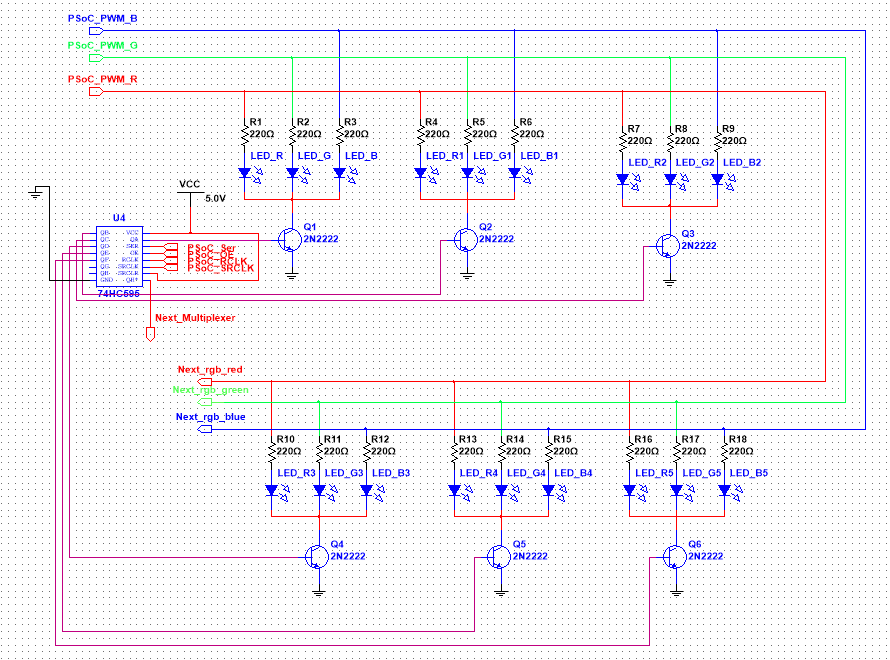
\includegraphics[width=\textwidth]{HardwareDesign/CupLight/graphics/CupLight.png}
    \caption{Hardware design af controller til CupLight, der anvender multiplexing}
    \label{fig:CupLight_HW_Multiplexing}
\end{figure}

\subsubsection{Styring uden multiplexing, ved ShiftRegister PWM}
En anden grund til at lige netop 74HC595 IC'en blev valgt er, at det med den også er muligt at styre lyset uden multiplexing. Den kan nemlig lade sig gøre at pulse width modulate de forskellige pins ud fra en algoritme, der sørger for at den sekvens af bit der bliver shiftet ind svarer til at en pin bliver anspændt med et bestemt PWM signal. Hvis denne implementeres, så skal der et lidt anderledes design, kan som ses på figur \ref{fig:CupLight_HW_ShiftPWM}
\begin{figure}[H]
    \centering
    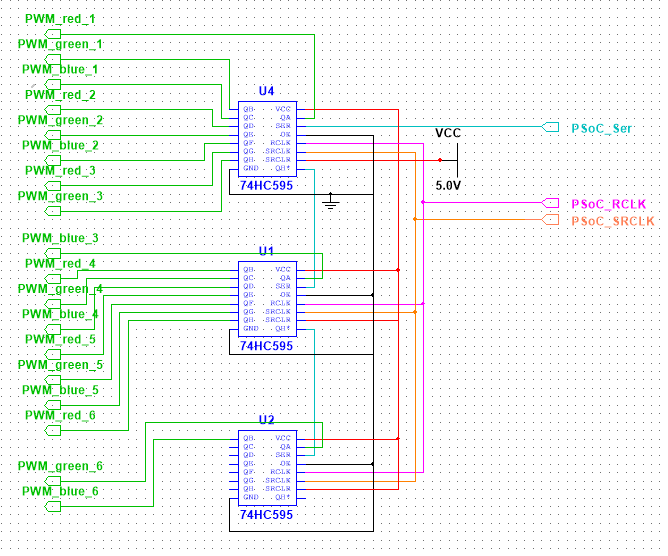
\includegraphics[width=\textwidth]{HardwareDesign/CupLight/graphics/CupLight_HW_Controller.png}
    \caption{Hardware design for CupLight controller, der anvender ShiftPWM}
    \label{fig:CupLight_HW_ShiftPWM}
\end{figure}

Denne form for controller simplificere  hardwaren, men gør softwaren mere krævende. Det gode ved denne implementering er som sagt, at timingen spiller en mindre væsentlig rolle og den kræver kun 3 pins på PSoC mod multiplexings 7.

Herudover skal der også laves et design til selve lyset på kop holderen. Den består af en PNP-transistor, der gør at strømmen ikke trækkes direkte fra PSoC'en, men en strømforsyning i stedet. Herudover består den af nogle 5 LED'er med tilhørende resistorer, der har værdier som tidligere beregnet. Alt dette ses i figur \ref{fig:CupHolder_HW}

\begin{figure}[H]
    \centering
    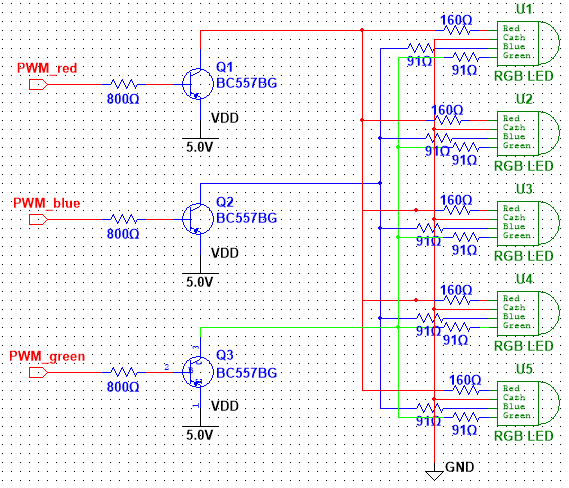
\includegraphics[width=\textwidth]{HardwareDesign/CupLight/graphics/CupHolder_HW.png}
    \caption{Hardware for Lyset i kop holderen}
    \label{fig:CupHolder_HW}
\end{figure}

\end{document}